%%%%%%%%%%%%%%%%%%%%%%%%%%%%%%%%%%%%%%%%%
% Beamer Presentation
% LaTeX Template
% Version 1.0 (10/11/12)
%
% This template has been downloaded from:
% http://www.LaTeXTemplates.com
%
% License:
% CC BY-NC-SA 3.0 (http://creativecommons.org/licenses/by-nc-sa/3.0/)
%
%%%%%%%%%%%%%%%%%%%%%%%%%%%%%%%%%%%%%%%%%

%----------------------------------------------------------------------------------------
%   PACKAGES AND THEMES
%----------------------------------------------------------------------------------------

\documentclass{beamer}
\usepackage{wrapfig}
\usepackage{amsmath}
\mode<presentation> {

% The Beamer class comes with a number of default slide themes
% which change the colors and layouts of slides. Below this is a list
% of all the themes, uncomment each in turn to see what they look like.

%\usetheme{default}
%\usetheme{AnnArbor}
%\usetheme{Antibes}
%\usetheme{Bergen}
%\usetheme{Berkeley}
%\usetheme{Berlin}
%\usetheme{Boadilla}
%\usetheme{CambridgeUS}
%\usetheme{Copenhagen}
%\usetheme{Darmstadt}
%\usetheme{Dresden}
%\usetheme{Frankfurt}
%\usetheme{Goettingen}
%\usetheme{Hannover}
%\usetheme{Ilmenau}
%\usetheme{JuanLesPins}
%\usetheme{Luebeck}
\usetheme{Madrid}
%\usetheme{Malmoe}
%\usetheme{Marburg}
%\usetheme{Montpellier}
%\usetheme{PaloAlto}
%\usetheme{Pittsburgh}
%\usetheme{Rochester}
%\usetheme{Singapore}
%\usetheme{Szeged}
%\usetheme{Warsaw}

% As well as themes, the Beamer class has a number of color themes
% for any slide theme. Uncomment each of these in turn to see how it
% changes the colors of your current slide theme.

%\usecolortheme{albatross}
%\usecolortheme{beaver}
%\usecolortheme{beetle}
%\usecolortheme{crane}
\usecolortheme{dolphin}
%\usecolortheme{dove}
%\usecolortheme{fly}
%\usecolortheme{lily}
%\usecolortheme{orchid}
%\usecolortheme{rose}
%\usecolortheme{seagull}
%\usecolortheme{seahorse}
%\usecolortheme{whale}
%\usecolortheme{wolverine}

%\setbeamertemplate{footline} % To remove the footer line in all slides uncomment this line
%\setbeamertemplate{footline}[page number] % To replace the footer line in all slides with a simple slide count uncomment this line

%\setbeamertemplate{navigation symbols}{} % To remove the navigation symbols from the bottom of all slides uncomment this line
}

\usepackage{graphicx} % Allows including images
\usepackage{booktabs} % Allows the use of \toprule, \midrule and \bottomrule in tables

%----------------------------------------------------------------------------------------
%   TITLE PAGE
%----------------------------------------------------------------------------------------

\title[Modern Software Development Practices]{Scientific Programming - A Motivation for Best Practice} % The short title appears at the bottom of every slide, the full title is only on the title page

\author{Ryan Pepper} % Your name
\institute[University of Southampton] % Your institution as it will appear on the bottom of every slide, may be shorthand to save space
{
University of Southampton \\ % Your institution for the title page
\medskip
\textit{ryan.pepper@soton.ac.uk} % Your email address
}
\date{October 29th 2018} % Date, can be changed to a custom date

\begin{document}

\begin{frame}
\titlepage % Print the title page as the first slide
\end{frame}

%\begin{frame}
%\frametitle{Overview} % Table of contents slide, comment this block out to remove it
%\tableofcontents % Throughout your presentation, if you choose to use \section{} and \subsection{} commands, these will automatically be printed on this slide as an overview of your presentation
%\end{frame}

%----------------------------------------------------------------------------------------
%   PRESENTATION SLIDES
%----------------------------------------------------------------------------------------

%------------------------------------------------
\section{Motivation} % Sections can be created in order to organize your presentation into discrete blocks, all sections and subsections are automatically printed in the table of contents as an overview of the talk
%------------------------------------------------

\begin{frame}
\frametitle{Current status}
\begin{itemize}
\item Expectation is that your scientific code must be error free.
\item Sources of errors can either be conceptual or in the implementation
\end{itemize}
\centering

What happens when things go wrong with software?
Let's start with a few high profile example...
\end{frame}

\begin{frame}
\frametitle{Geoffrey Chang}

\begin{columns}
\begin{column}{0.7\textwidth}
\begin{itemize}
\item Geoffrey Chang and coauthors published a series of papers in high profile journals (Science, Nature) which attempted
to determine the structure of molecules through analysing X-Ray crystallography data 
\item Papers very highly cited.
\item However, in 2006 Kasper Locher solved problem for similar crystal but found 180 flip in helix suggesting that the results were incorrect
\item Chang used his own software to analyse the data.
\item Two columns accidentally transposed in a table which resulted in the signs of charges in the structure being flipped.
\item This led to retraction of 6 papers - 5 years of work.
\end{itemize}
\end{column}

\begin{column}{0.3\textwidth}
    \begin{figure}
        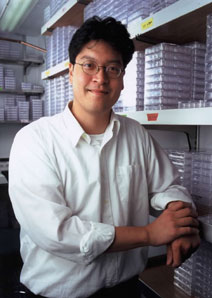
\includegraphics[width=0.95\columnwidth]{images/chang_jeff.jpg}
    \end{figure}
\end{column}
\end{columns}
\end{frame}



\begin{frame}
\frametitle{Reinhart and Rogoff}
\begin{columns}
    \begin{column}{0.325\textwidth}
        \begin{figure}
            
\includegraphics[width=\columnwidth]{images/reinhart.png}
        \end{figure}
    \end{column}

    \begin{column}{0.675\textwidth}
        \begin{itemize}
            \item Widely cited paper "Growth in a time of Debt" by Reinhart and Rogoff (former chief economist of IMF) in politics and economics on effectiveness of austerity.
            \item Studied effect of debt ratio to GDP and argued growth declined once $> 60\%$.Used as evidential basis for austerity budgets by EU Commissioner Olli Rehn, UK Chancellor George Osborne, Republican Party in USA.
            \item Herndon, et. al. requested the non-public data and were given it by authors, and found spreadsheet errors.
            \item Fixing errors showed that historical decline in growth once a countries GDP reached certain debt levels was not as high as claimed.
        \end{itemize}
    \end{column}
\end{columns}
\end{frame}

\begin{frame}
    \frametitle{Ariane 5 Rocket Launch 1996}
    \begin{columns}
        \begin{column}{0.35\textwidth}
            \begin{figure}
                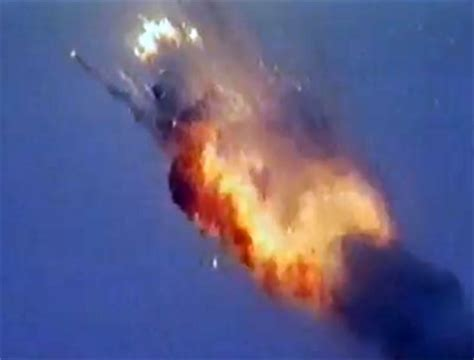
\includegraphics[width=\columnwidth]{images/ariane5.jpeg}
            \end{figure}
        \end{column}
    
        \begin{column}{0.65\textwidth}
            \begin{itemize}
                \item 10 year development and \$7 Billion cost for European Space Agency
                \item First test launch in June 1996. 37 seconds after launch, trajectory went off course and self destruct mechanism kicked in.
                \item Inertial reference system had software bug.
                \item Conversion of a 64-bit float into a 16-bit integer caused integer overflow.
                \item Reused software from Ariane 4 but this rocket reached much higher speeds so rocket attempted to make correction for altitude deviation which hadn't happened.
                \item Worst part was that this part of code was no longer needed for Ariane 5!
            \end{itemize}
        \end{column}
    \end{columns}
\end{frame}

\begin{frame}
    \frametitle{NHS Connecting for Health}
    \begin{itemize}
        \item No national NHS health records database
        \item Government awarded contracts to Accenture, Fujitsu, BT Health and Computer Sciences Corporation between  2002 and 2004 to 5 build regional systems which could integrate with one another within 3 years. 
        \item Proposed system had expected cost \textsterling 2.3 Billion and would have been biggest IT project in the world.
        \item Scheme cancelled in 2011 but 16 years later costs from fallout of this project still escalating - currently over \textsterling 20 billion (c.f. entirity of UK science funding in 2018 is \textsterling 5 billion).
        \item Government report "Government and IT - a recipe for rip offs" in 2011 blamed \textbf{lack of in-house technical knowledge} and a \textbf{tendency to build large complex projects that cannot adapt to changing requirements}.
    \end{itemize}
\end{frame}

\begin{frame}
    \frametitle{More examples}
    \begin{itemize}
        \item Trading glitch cost Knight Capital \$440 Million dollars in 30 minutes.
        \item Therac-25 Radiation Therapy machine bug killed 4 patients and injured two others because of integer overflow in software written by a single programmer.
        \item Mars Orbiter crashed in 1998 because of imperial vs metric units in interface between software.
        \item Y2K bug was caused by 32-bit integer commonly used to store dates overflowing.
        \item 1999 Study on suicides after natural disasters counted deaths in one year twice and had to be retracted.
        \item Sainsbury's wrote off \$526 Million investment in 2004 because of software bugs.
    \end{itemize}
\end{frame}

\begin{frame}
    \frametitle{Implications of badly written software}
    \begin{itemize}
    \item Complex systems are very hard to get right.
    \item Getting it wrong for you means bad science and a damaged career.
    \item If you work on large projects it can mean huge costs.
    \item Wasted time and money dealing with fallout of mistakes.
    \item Poorly designed software is just as bad as bugs in well designed software!
    \end{itemize}
\end{frame}

\begin{frame}
    \frametitle{What should we draw from this?}
    \begin{itemize}
        \item Clear that even professional software developers can get it wrong.
        \item Scientists in particular are not generally good programmers and are mostly self taught.
        \item Scientists do not have the resources to use all of the techniques from industry to avoid problems.
    \end{itemize}
\end{frame}

\begin{frame}
    \frametitle{Reproducibility and Repeatability}
    \begin{itemize}
        \item \textbf{Reproducibility - Gaining results which are close in agreement using the same methodology described}
        \item Key concept of the scientific method
        \item \textbf{Often scientific papers cannot be reproduced} from the paper alone.
        \item How many of you have ever struggled to reproduce a result from a computational paper?
        \item Often this comes from inherent assumptions in modelling which are not discussed in the research literature itself.
        \item Very challenging to write a paper which is complete.
        \item Large and well discussed "reproducibility crisis"
    \end{itemize}
\end{frame}

\begin{frame}
    \frametitle{A Changing Landscape?}
    \begin{itemize}
        \item Increasing pressure from funders - all UK research data must be made public. Similar story in other countries.
        \item However, papers and the data are still are not generally enough to reproduce methods.
        \item Organisations like the Software Sustainability Institute and Software Carpentry have been leads in giving scientists better software development training.
        \item Well written open projects in Python/C/Fortran like AstroPy, SciPy and NumPy are well documented and serve as great examples for writing well tested and usable software.
        \item Time commitment to getting there is hard at first but leads you to do better science and have more confidence in your results.

    \end{itemize}
\end{frame}

\begin{frame}
\frametitle{A Changing Landscape?}
%    \centering
    It is becoming increasingly necessary for you to release the source code that generates your publications. It is highly likely you won't be able to decline in future! For e.g.:
    \begin{figure}
        
\includegraphics[width=0.5\textwidth]{images/Nature-guidelines.png}
    \end{figure}
    
\end{frame}
\begin{frame}
    \frametitle{Best Practice - What are we going to learn?}
    Everything here is absolutely essential to writing good software - in industry these just starting points from which all else follows.
    If you are not doing any one of these things, you are almost certainly not writing good software.

    It's also worth saying that doing these things does not mean you'll write good software either, but it's less likely to be really terrible...

    \begin{itemize}
        \item Reproducible environment - laying out how to build software in a way others can follow through using containers.
        \item Keeping a history of your code - often we need to revert back to old versions or look at where bugs were introduced. Version control helps us do this.
        \item Testing and Continuous Integration - Tests let you know when something has broken unexpectedly. Continuous Integration runs tests consistently every time you make changes.
        \item Writing Documentation - A practical guide.
    \end{itemize}
\end{frame}

\end{document}